\documentclass{article}
\usepackage[utf8]{inputenc}

\title{Fibonacci Sequence and Golden Ratio Connection}
\author{Connor Scholten}
\date{July 2020}

% Packages
\usepackage[utf8]{inputenc}     % Unicode input 
\usepackage{amsmath, amssymb}   % American Math Society Foratting & Symbols
\usepackage{graphicx}           % Allows you to insert graphics
\usepackage{hyperref}           % Allows automatic references & hyperlinking
\usepackage{indentfirst}

% Macros (these are shortcuts)
% Read more about them here 
% http://www.math.uh.edu/~torok/math_6298/latex/macros.html
\newcommand{\R}{{\mathbb R}}    % Type $\R$ instead of $\mathbb{R}$ for the real numbers styliezed R
\newcommand{\vt}{\mathbf}       % Type $\vt{...}$ instead of $\mathbf{...}$ to bold a symbol.

\begin{document}

\maketitle

\section{Introduction}

Fibonacci sequence is named after Italian mathematician Leonardo of Pisa, later known as Fibonacci. In his 1202 book Liber Abaci, Fibonacci introduced the sequence to Western European mathematics, although the sequence had been described earlier in Indian mathematics, or as early as 200 BC in work by Pingala on enumerating possible patterns of Sanskrit poetry formed from syllables of two lengths. \\

Fibonacci numbers appear unexpectedly often in mathematics, so much so that there is an entire journal dedicated to their study, the Fibonacci Quarterly. One of early most notable is the classic Fibonacci rabbit reproduction problem. Consider two newborn rabbits are placed in a pen, how many rabbits will there be in one year? This is assuming rabbits always produce exactly one male and female offspring, can reproduce once every month, can start to reproduce once they are one month old, and they will never die. \\

Basically we run through the first few months until we feel to have locked on the pattern. We will count the rabbits in pairs. The start, or the 0th month, there is one pair of newborn rabbits. The 1st month there is one pair, but now they are old enough to reproduce. The 2nd month there is a birth of a second pair with one adult pair and one newborn pairing. Now the 3rd month the original pair give birth again and now the second pair are adults, so we are at 3, the 4th month those two adult pair give birth and now we are at 5 pairs, 3 adults and 2 newborn pairs, the 6th month will be adding the 5 pairs with the extra 3 that will give birth since we had 3 adult pairs last round, this gives a sequence of

\begin{equation*}
    1,1,2,3,5,8,\ldots
\end{equation*}

The underlying pattern seems to come from adding the previous 2 numbers in the sequence, this is because the term that we are on is based on the number of pairs last round, the round before that will count how many adult pairs can give birth, thus we have our recurrence of $a_n=a_{n-1}+a_{n-2}$ with $a_0=a_1=1$, continuing this we eventually get to the 12th month of 
\begin{equation*}
    1, 1, 2, 3, 5, 8, 13, 21, 34, 55, 89, 144, \underbrace{233}_{12th}, 377, \ldots 
\end{equation*}

Stated as 233 pairs or 466 Rabbits in the pen. \\

This sequence and recursion is the Fibonacci sequence.  With the recursion we also stated two initial values, or in computer science they would be called base cases. If we changed those values the sequence would come out very differently, for example, with $a_0=1, a_1=3$, essentially we put a pair in the pen, then end of first month we put two more newborn pairs in the pen, then let them go nuts. We will see the sequence with this yet same recurrence but different basis comes out to be what is called the Lucas sequence

\begin{equation*}
    1,3,4,7,11,18,29,47,76,123,199,\ldots
\end{equation*}

\section{Golden Ratio}

The Golden Ratio is a constant in mathematics, it is an irrational number usually abbreviated using the letter, $\varphi$. Mostly used in the realm of Architecture for the ascetically pleasing look of it, but shows up in music and other art forms. It is described by the relationship

\begin{figure*}[!htbp]
\centering
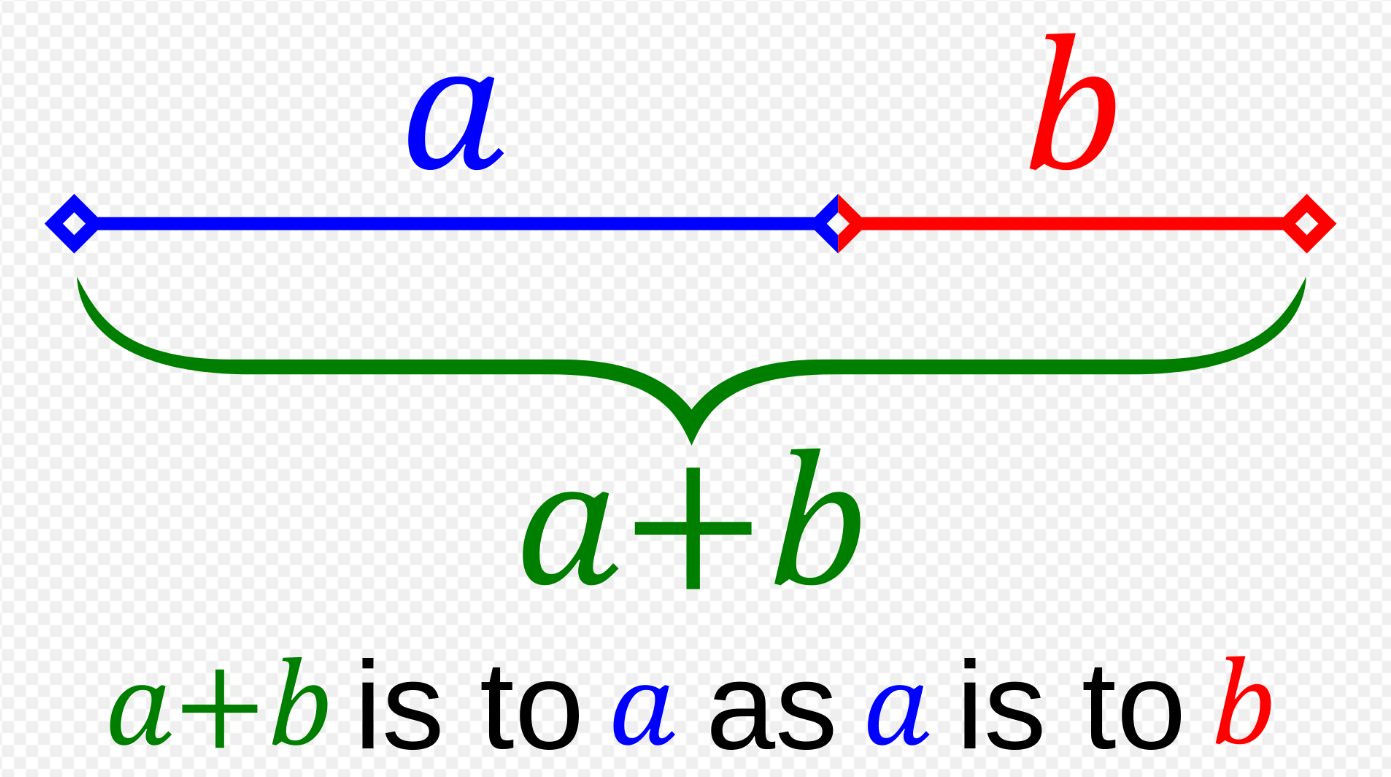
\includegraphics[scale=.2]{Golden.PNG}
\label{fig:3}
\end{figure*}

The relationship of the ratio from small part to big part being the same as the ratio from the big part to the whole thing ends up being a constant. Realize with the letters involved this makes an equation of $\frac{a}{b}=\frac{a+b}{a}=\varphi$, this will turn into

\begin{align*}
    \frac{a}{b}&=\frac{a+b}{a} \\
    a^2&=ab+b^2 
\end{align*}

We will initially set $b=1$ so it becomes one equation and one unknown, after seeing the argument try running through the argument again with whatever various values of $b$ you desire and we would see the result remains unchanged. Now we have a polynomial that obtains the Golden Ratio

\begin{align*}
    a^2=a+1& \\
    a^2-a-1&=0 \\
    a=\frac{1 \pm \sqrt{5}}{2}.
\end{align*}

Realize that $\frac{a}{b}=\varphi$ with $b=1$ so $a=\varphi=\frac{1 \pm \sqrt{5}}{2}$. However note that $\frac{1+\sqrt{5}}{2}\approx 1.618033$ and $\frac{1-\sqrt{5}}{2}\approx -0.118033$. Having a negative ratio to describe the multiplier of two line lengths doesn't make physical sense so we will finally state the real golden ratio is $\varphi \approx 1.618033$. Also realize it came from the polynomial $x^2-x-1=0$ so if we see that polynomial we will know the golden ratio is the answer. We will be using the negative root answer in other problems without that physical context constraint. We will be calling it $\overline{\varphi}$. We will show $\overline{\varphi}=1-\varphi$, which can be a nice relationship between the two

\begin{align*}
    \overline{\varphi} &= 1-\varphi \\
     &= 1-\frac{1+\sqrt{5}}{2} \\
     &= \frac{2-(1+\sqrt{5})}{2} \\
     &= \frac{1 - \sqrt{5}}{2} \\
     &= \overline{\varphi}.
\end{align*}

We can also manipulate that equation with some adds and subtracts to also be $\varphi=1-\overline{\varphi}$.

\section{Explicit formula}

There is a drawback to recurrence relations, that is being tough to calculate terms in the future, for example what if we wanted to find the 100th Fibonacci number? We would have to continue to type and calculate for a solid few minutes, one new term at a time until we arrived at the number 354,224,848,179,261,915,075. Then imagine how bad it would be to calculate the 1000th Fibonacci number. This leads to the concept of finding what is called an explicit or a closed formula. The Fibonacci closed formula will be a special one since it gets to have the Golden Ratio in it. \\

To hint why it will have the Golden Ratio, notice how if we take division of successive numbers in the Fibonacci sequence and watch them approach $\varphi \approx 1.618033$

\begin{align*}
    \frac{1}{1}=1 \quad \frac{2}{1}=2 \quad \frac{3}{2}=1.5 &\quad \frac{5}{3}\approx1.666 \quad \frac{8}{5}=1.6 \quad \frac{13}{8}=1.625 \\
    \frac{21}{13}\approx1.6153 \quad \frac{34}{21}\approx1.6190 &\quad \frac{55}{34}\approx1.6176 \quad \frac{89}{55}\approx1.6181 \quad \frac{144}{55}\approx1.61798. \\
\end{align*}

We will find the closed formula with three methods, the first is a guess and check, Fibonacci is a recurrence relation that is in a category called 2nd order Linear difference equation. The parallel between it and second order linear Differential Equations is uncanny. \\

The second way needs Linear Algebra to solve. We will show that we can find the closed formula by rewriting it as an Eigenvalue-Eigenvector problem to build a matrix Diagonalization to find powers of a matrix that calculates terms recursively. \\

The third way involves Taylor Series, through creating the Fibonacci Generating Function from the recurrence, then solving that for the answer.

\subsection{Guess and Check with Superposition Principle}

In here we will use initial values $a_0=0, a_1=1$. This will create the same sequence using the same recursion but the indexing will be different by being off by one, compared to the last time we stated the initial values above. Having $a_0=0$ makes it easier to derive a closed form here. \\

Just like in Second Order Linear Differential Equations, we will guess a trial solution of $x^n$ and see how it works out. So with $a_n=x^n$

\begin{align*}
    a_n=a_{n-1}+a_{n-2}& \text{ with } a_0=0, a_1=1 \\
    x^n=&x^{n-1}+x^{n-2} \\
       =&x^{n-2}(x+1).
\end{align*}

By laws of exponents realize that $x^n=x^{n-2}x^2$, so notice how that means we need $x^2=(x+1)$ to line up with our equation, these will make the solutions. Thus we have to solve the polynomial of $x^2-x-1=0$, but this is the Golden Ratio Polynomial we did earlier, thus the answer is either $\frac{1+\sqrt{5}}{2}$, or $\frac{1-\sqrt{5}}{2}$, aka $\varphi$ and $\overline{\varphi}$. \\

Now we take the superposition principle as $a_n=c_0 (\varphi)^n + c_1 (\overline{\varphi})^n$, we have two constants but we also have initial values to satisfy. So $a_0=a_1=1$ means that

\begin{align*}
    a_0=0&=c_0+c_1 \\
    a_1=1&=c_0(\varphi)^1+c_1(\overline{\varphi})^1.
\end{align*}

Thus we solve via a substitute $c_0=-c_1$ to get $1=(-c_1)(\varphi)+c_1(\overline{\varphi})$. Using our $\overline{\varphi}=1-\varphi$ makes

\begin{align*}
    1=&(-c_1)(\varphi)+c_1(1-\varphi) \\
    1=&-c_1\varphi+c_1-c_1\varphi \\
    1=&-2c_1\varphi+c_1 \\
    1=&c_1(1-2\varphi) \\
    c_1=& \frac{1}{1-2\varphi}.
\end{align*}

Recall and sub $\varphi$ back to get $\frac{1}{1-2\left(\frac{1+\sqrt{5}}{2}\right)}=\frac{1}{1-1+\sqrt{5}}=\frac{1}{\sqrt{5}}$. This means $c_1=\frac{1}{\sqrt{5}}$ and to ensure the zero equation $c_2=-\frac{1}{5}$. This makes a final closed form solution of 

\begin{equation*}
    a_n=\frac{1}{\sqrt{5}} (\varphi)^n - \frac{1}{\sqrt{5}} (\overline{\varphi})^n.
\end{equation*}

\subsection{Matrix Derivation}

This is a rather clever method to find the formula, it is more systematic than just a lucky guess of $x^n$ like last round. However it takes many more advanced Linear Algebra concepts to make up for that lucky guess. We will start with setting up a Matrix Equation and we will use it to find the explicit formula for $a_n=a_{n-1}+a_{n-2}$. We will define

\begin{equation*}
    A=\begin{bmatrix}
        1 & 1 \\
        1 & 0
    \end{bmatrix}
\end{equation*}

Then we also define $\vec{x_n}=\begin{bmatrix} a_{n+1} \\ a_n \end{bmatrix}$, the bottom entry of this vector will be the key that stores the closed formula eventually. Notice that 

\begin{align*}
    A\vec{x_n}&=A=\begin{bmatrix}
        1 & 1 \\
        1 & 0
    \end{bmatrix} \begin{bmatrix} a_{n+1} \\ a_n \end{bmatrix} \\
    =& \begin{bmatrix} a_n+a_{n+1} \\ a_{n+1} \end{bmatrix} \\
    =& \begin{bmatrix} a_{n+2} \\ a_{n+1} \end{bmatrix}.
\end{align*}

That means multiplying $A$ will increase the vector to the next numbers in the Fibonacci Sequence, meaning in general

\begin{equation*}
    \vec{x_n}=A^n\vec{x_0} \text{ where } \vec{x_0}=\begin{bmatrix} 1 \\ 0 \end{bmatrix}.
\end{equation*}

So in order to calculate $A^n$ we will want to Diagonalize to shortcut the calculation if we can. Meaning we will need to find Eigenvalues and Eigenvectors of the Matrix

\begin{equation*}
    A=\begin{bmatrix}
        1 & 1 \\
        1 & 0
    \end{bmatrix}
\end{equation*}

To find the Eigenvalues we have to solve the characteristic equation $det(A-\lambda I) = 0$, where

\begin{equation*}
    \lambda I=\begin{bmatrix}
        \lambda & 0 \\
        0 & \lambda
    \end{bmatrix}
\end{equation*}

which makes

\begin{equation*}
    A-\lambda I=\begin{bmatrix}
        1-\lambda & 1 \\
        1 & -\lambda
    \end{bmatrix}.
\end{equation*}

Then $det(A-\lambda I)=0$ leads to $(1-\lambda)(-\lambda)-1=0$, or that $\lambda^2-\lambda -1=0$. Notice this is the golden ratio polynomial. So we will skip to the answer and find Eigenvalues $\lambda_1=\varphi$ and $\lambda_2=\overline{\varphi}$. \\

Now time to find the Eigenvectors using $A-\lambda_1I=\mathbf{0}$ and $A-\lambda_2I=\mathbf{0}$. Starting with $\lambda_1=\varphi$, we will have

\begin{equation*}
    A-\lambda_1 I =
    \begin{bmatrix}
        1-\lambda_1 & 1 \\
        1 & -\lambda_1
    \end{bmatrix} = 
    \begin{bmatrix}
        1-\varphi & 1 \\
        1 & -\varphi
    \end{bmatrix}
\end{equation*}

Row reducing, we will take advantage by a row swap then do a replacement subtract Row 1 multiplied by $(1-\varphi)$ then subtract Row 2. Then notice how $(-\varphi(1- \varphi))-1=\varphi^2-\varphi-1$, this makes zero since $\varphi$ is a solution to this quadratic, this gets an R.R.E.F. of

\begin{align*}
    \left[ \begin{array}{cc|c} 1- \varphi & 1 & 0 \\ 1 & -\varphi & 0 \end{array} \right] &\sim \left[ \begin{array}{cc|c}  1 & -\varphi & 0 \\ 1-\varphi & 1 & 0 \end{array} \right] \\
    &\sim \left[ \begin{array}{cc|c}  1 & -\varphi & 0 \\ (1-\varphi)- (1-\varphi) & (-\varphi(1- \varphi))-1 & 0 \end{array} \right] \\
    &\sim \left[ \begin{array}{cc|c} 1 &  -\varphi & 0 \\ 0  & 0 & 0 \end{array}  \right]
\end{align*} 

Writing out top row as equation, we obtain

\begin{align*}
    x_1 &-\varphi x_2 = 0\\
    x_1 &= \varphi x_2.
\end{align*}

This makes the Eigenvector

\begin{equation*}
    \begin{bmatrix} x_1 \\ x_2 \end{bmatrix} = \begin{bmatrix} \varphi x_2 \\ x_2 \end{bmatrix} = x_2 \begin{bmatrix} \varphi \\ 1 \end{bmatrix}.
\end{equation*}

This means $v_1=\begin{bmatrix} \varphi \\ 1 \end{bmatrix}$ is the Eigenvector of value $\lambda_1=\varphi$. \\

For $\lambda_2=1-\varphi=\overline{\varphi}$, the calculations will carry out the same way, except all $\varphi$ will be replaced with $1-\varphi$ or $\overline{\varphi}$. Note the symmetry of $1-\varphi=\overline{\varphi}$ can be restated as $1-\overline{\varphi}=\varphi$. Thus, the row reduced augmented matrix would similarly be 

\begin{align*} \left[ \begin{array}{cc|c} 1 &  \varphi-1 & 0 \\ 0  & 0 & 0 \end{array}  \right] \end{align*}

Writing out top row as equation,

\begin{align*}
    x_1 &+(\varphi-1) x_2 = 0\\
    x_1 &= (1-\varphi) x_2.
\end{align*}

This makes the Eigenvector

\begin{equation*}
    \begin{bmatrix} x_1 \\ x_2 \end{bmatrix} = \begin{bmatrix} (1-\varphi) x_2 \\ x_2 \end{bmatrix} = x_2 \begin{bmatrix} (1-\varphi) \\ 1 \end{bmatrix}.
\end{equation*}

This means $v_2=\begin{bmatrix} 1-\varphi \\ 1 \end{bmatrix}$ is the Eigenvector of value $\lambda_2=1-\varphi$. \\

Since we have now have the needed Eigeninformation of $A$, we can successfully Diagonalize the matrix. $A = PDP^{-1}$, $P$ is the matrix formed by the Eigenvectors, $D$ is the diagonal matrix, where the values in each column correspond to the Eigenvectors represented in $P$, and $P^{-1}$ is the inverse of $P$. Thus,

\begin{equation*}
    P = \begin{bmatrix}
            \varphi & 1-\varphi \\
             1 & 1
        \end{bmatrix} \qquad \text{and} \qquad
    D = \begin{bmatrix}
            \varphi & 0 \\
            0 & 1-\varphi
        \end{bmatrix}.
\end{equation*}

Then $A=PDP^{-1}$ looks like

\begin{equation*}
    \begin{bmatrix}
        1 & 1 \\
        1 & 0
    \end{bmatrix} =
    \begin{bmatrix}
        \varphi & 1-\varphi \\
        1 & 1
    \end{bmatrix}
    \begin{bmatrix}
        \varphi & 0 \\
        0 & 1-\varphi
    \end{bmatrix}
    \begin{bmatrix}
        \varphi & 1-\varphi \\
        1 & 1
    \end{bmatrix}^{-1}.
\end{equation*}


We know that $\vec{x_n} = A^n \vec{x_0}$, where $\vec{x_n}=\begin{bmatrix} a_{n+1} \\ a_n \end{bmatrix}$ and $a_n$ is $n$th term of the Fibonacci sequence. This makes $x_0 = \begin{bmatrix} a_{1} \\ a_0 \end{bmatrix}=\begin{bmatrix} 1 \\ 0 \end{bmatrix}$. We also have a Diagonalization of $A$ so now we have a means of calculating the $A^n$. Since $A=PDP^{-1}$, then $A^2=PDP^{-1}PDP^{-1}= PD^2P^{-1}, A^3=PD^2P^{-1}\cdot PDP^{-1} = PD^3P^{-1}$, and so on. Thus, $A^n = PD^nP^{-1}.$ \\

Plugging this into the $\vec{x_n}$ formula, we see $\vec{x_n} = PD^nP^{-1} \vec{x_0}$, or 

\begin{equation*}
   \vec{x_n} =
     \begin{bmatrix}
        \varphi & 1-\varphi \\
        1 & 1
    \end{bmatrix}
    \begin{bmatrix}
        \varphi^n & 0 \\
        0 & (1-\varphi)^n
    \end{bmatrix}^n
    \begin{bmatrix}
        \varphi & 1-\varphi \\
        1 & 1
    \end{bmatrix}^{-1}
    \begin{bmatrix}
    1\\0
    \end{bmatrix}.
\end{equation*}
    
Also, in order to calculate the $P^{-1}$ matrix, remember that the inverse of a 2 $\times$ 2 matrix 
$\begin{bmatrix}
a & b\\
c & d
\end{bmatrix}$ 
can be found by the formula 

\begin{equation*}
   \begin{bmatrix}
   a & b \\
   c & d
   \end{bmatrix}^{-1} = \frac{1}{ad-bc} \begin{bmatrix}
    d & -b \\
    -c & a
    \end{bmatrix}
\end{equation*}

Thus, 

\begin{align*}
    \begin{bmatrix}
        \varphi & 1-\varphi \\
        1 & 1
    \end{bmatrix}^{-1} &= \frac{1}{\varphi-(1-\varphi)} \begin{bmatrix}
    1 & -(1-\varphi)\\
    -1 & \varphi
    \end{bmatrix} \\
    &= \frac{1}{2\varphi-1} \begin{bmatrix}
    1 & \varphi-1\\
    -1 & \varphi
    \end{bmatrix}
\end{align*}

Remembering that $\varphi = \frac{1+\sqrt{5}}{2}$, we see \begin{align*}
    \frac{1}{2\varphi -1 } &= \frac{1}{2 (\frac{1+\sqrt{5}}{2}) -1} \\
    &= \frac{1}{1+\sqrt{5} -1} \\
    &= \frac{1}{\sqrt{5}}
\end{align*}

Then, we conclude that $P^{-1} = \frac{1}{\sqrt{5}} \begin{bmatrix}
    1 & \varphi-1\\
    -1 & \varphi
    \end{bmatrix}$, and that
    
\begin{equation*}
     \vec{x_n} = \frac{1}{\sqrt{5}}
     \begin{bmatrix}
        \varphi & 1-\varphi \\
        1 & 1
    \end{bmatrix}
    \begin{bmatrix}
        \varphi^n & 0 \\
        0 & (1-\varphi)^n
    \end{bmatrix}
    \begin{bmatrix}
    1 & \varphi-1\\
    -1 & \varphi
    \end{bmatrix}
    \begin{bmatrix}
    1\\0
    \end{bmatrix} 
    \end{equation*}
    
Multiplying this equation out,
    \begin{align*}
        \vec{x_n} &= \frac{1}{\sqrt{5}} \cdot \begin{bmatrix}
        \varphi^{n+1} & (1-\varphi)^{n+1} \\
        \varphi^n & (1-\varphi)^n
    \end{bmatrix} \begin{bmatrix}
    1 & \varphi-1\\
    -1 & \varphi
    \end{bmatrix} \begin{bmatrix}
    1\\0
    \end{bmatrix} \\
    &= \frac{1}{\sqrt{5}} \cdot \begin{bmatrix}
    \varphi^{n+1} - (1-\varphi)^{n+1} & \varphi^{n+1}(\varphi-1) + \varphi(1-\varphi)^{n+1} \\
    \varphi^n - (1-\varphi)^n & \varphi^n(\varphi -1) +\varphi(1-\varphi)^n
    \end{bmatrix} \begin{bmatrix}
    1\\0
    \end{bmatrix} \\
    &= \frac{1}{\sqrt{5}} \cdot \begin{bmatrix}
     \varphi^{n+1} - (1-\varphi)^{n+1} \\
      \varphi^n - (1-\varphi)^n
    \end{bmatrix} \\
    &=  \begin{bmatrix}
     (\frac{1}{\sqrt{5}})\varphi^{n+1} - \frac{1}{\sqrt{5}}(1-\varphi)^{n+1} \\
      (\frac{1}{\sqrt{5}})\varphi^n - \frac{1}{\sqrt{5}}(1-\varphi)^n
    \end{bmatrix}
\end{align*}

We remind ourselves that the bottom entry of this matrix corresponded to $a_n$. We now found yet again the closed formula

\begin{equation*}
    a_n = \frac{1}{\sqrt{5}} \left(\frac{1+\sqrt{5}}{2} \right)^n - \frac{1}{\sqrt{5}} \left(\frac{1-\sqrt{5}}{2} \right)^n.
\end{equation*}

\subsection{Generating Functions.}

A Generating Function approach is also systematic and only takes the a background of understanding Taylor Series and Calculus II level topics instead of Linear algebra. It will however be filled with clever trickery to keep the story moving. If you have not worked with Generating Functions before you should read up on it on the Generating Function document first. We start with the recurrence, $a_0=0$, $a_1=1$ and use Generating Function $A(x)=\sum_{n=0}^{\infty}a_nx^n$. We will put in the work to find the closed form of that infinite polynomial as

\begin{align*}
    a_n &= a_{n-1}+a_{n-2} \\
    0 &= a_n-a_{n-1}-a_{n-2} \\
    \sum_{n=2}^{\infty} 0 &= \sum_{n=2}^{\infty} (a_n-a_{n-1}-a_{n-2})x^n \\
    0 &= \sum_{n=2}^{\infty}a_nx^n-x\sum_{n=2}^{\infty}a_{n-1}x^{n-1}-x^2\sum_{n=2}^{\infty}a_{n-2}x^{n-2} \\
    0 &= [A(x)-a_0-a_1x]-[x(A(x)-a_0)]-[x^2(A(x))] \\
    0 &= A(x)-x-xA(x)-x^2A(x) \\
    0 &= (1-x-x^2)A(x)-x \\
    A(x) &= \frac{x}{1-x-x^2}.
\end{align*}

With this, we have a Generating Function, consider that $1-x-x^2=0$ multiply by $-1$ has the same roots as $x^2+x-1=0$, we are not quite on the same golden ratio polynomial since the middle term has opposite sign so we quadratic to get almost the golden ratios.

\begin{equation*}
    x=\frac{-1 \pm \sqrt{5}}{2}.
\end{equation*}

Let's call $k_0=\frac{-1+\sqrt{5}}{2}$ and $k_1=\frac{-1-\sqrt{5}}{2}$. By having the roots we can claim an identity $(x-k_0)(x-k_1)=x^2-x-1$. For those that do not believe this, here is the algebra check for it.

\begin{align*}
    (x-k_0)(x-k_1)=&x^2-(k_0+k_1)x+k_0\cdot k_1 \\
                  =&x^2-\left(\frac{-1+\sqrt{5}}{2}+\frac{-1-\sqrt{5}}{2}\right)x+\frac{(-1+\sqrt{5})}{2}\frac{(-1-\sqrt{5})}{2} \\
                  =&x^2-\frac{2}{2}x+\frac{(-1+\sqrt{5})(-1-\sqrt{5})}{4} \\
                  =&x^2-x+\frac{1-(\sqrt{5})^2}{4} \\
                  =&x^2-x-1.
\end{align*}

That means we can substitute $1-x-x^2=-(x-k_0)(x-k_1)$

\begin{align*}
    A(x)&=\frac{x}{1-x-x^2} \\
        &=-\frac{x}{(x-k_0)(x-k_1)}.
\end{align*}

Next is partial fraction decomposition. Note the setup $\frac{x}{(x-k_0)(x-k_1)}=\frac{A}{(x-k_0)}+\frac{B}{(x-k_1)}$. By the cover up method we will obtain $A=\frac{k_0}{k_0-k_1}$ and $B=\frac{k_1}{k_1-k_0}$. To simplify, lets see that $k_0-k_1=\frac{-1+\sqrt{5}}{2}-\frac{-1-\sqrt{5}}{2}=\sqrt{5}$, this makes $A=\frac{k_0}{\sqrt{5}}$ and $B=\frac{k_1}{-\sqrt{5}}$. Now we are at

\begin{align*}
    A(x)&=-\frac{x}{(x-k_0)(x-k_1)} \\
        &=-\left(\frac{\frac{k_0}{\sqrt{5}}}{(x-k_0)}+\frac{\frac{k_1}{-\sqrt{5}}}{(x-k_1)}\right) \\
        &=\frac{1}{\sqrt{5}}\frac{k_1}{(x-k_1)}-\frac{1}{\sqrt{5}}\frac{k_0}{(x-k_0)} \\
        &=\frac{1}{\sqrt{5}}\frac{k_0}{(k_0-x)}-\frac{1}{\sqrt{5}}\frac{k_1}{(k_1-x)} \\
        &=\frac{1}{\sqrt{5}}\frac{1}{(1-\frac{1}{k_0}x)}-\frac{1}{\sqrt{5}}\frac{1}{(1-\frac{1}{k_1}x)}.
\end{align*}

We are now close enough in form to now take advantage of the Geometric Series $\frac{1}{1-x}=1+x+x^2+x^3\ldots=\sum_{i=0}^{\infty} x^i$. We can modify via substitutions with $x$ turning into $\frac{1}{k_0}x$ and $\frac{1}{k_1}x$ to get $\frac{1}{(1-\frac{x}{k_0})}=\sum_{i=0}^{\infty} \frac{1}{k_0^i}x^i$ and $\frac{1}{(1-\frac{x}{k_1})}=\sum_{i=0}^{\infty} \frac{1}{k_1^i}x^i$. Substitute and obtain

\begin{align*}
    A(x)&=\frac{1}{\sqrt{5}}\frac{1}{(1-\frac{1}{k_0}x)}-\frac{1}{\sqrt{5}}\frac{1}{(1-\frac{1}{k_1}x)} \\
        &=\frac{1}{\sqrt{5}}\sum_{i=0}^{\infty} \frac{1}{k_0^i}x^i-\frac{1}{\sqrt{5}}\sum_{i=0}^{\infty} \frac{1}{k_1^i}x^i \\
        &=\sum_{i=0}^{\infty} \frac{1}{\sqrt{5}} \frac{1}{k_0^i}x^i+\sum_{i=0}^{\infty}\frac{-1}{\sqrt{5}} \frac{1}{k_1^i}x^i \\
        &=\sum_{i=0}^{\infty} \left[\frac{1}{\sqrt{5}} \frac{1}{k_0^i}+\frac{-1}{\sqrt{5}} \frac{1}{k_1^i}\right]x^i \\
\end{align*}

Recall how we stated the Generating function is $A(x)=\sum_{n=0}^{\infty}a_nx^n$, aside from a different index variable, we are now perfectly lined up. Meaning we equate the $a_n$ coefficients to make the closed formula for a third and final time.

\begin{align*}
    a_n &=\frac{1}{\sqrt{5}} \frac{1}{k_0^n}+\frac{-1}{\sqrt{5}} \frac{1}{k_1^n} \\
        &=\frac{1}{\sqrt{5}} \left(\frac{1}{\frac{-1+\sqrt{5}}{2}}\right)^n+\frac{-1}{\sqrt{5}} \left(\frac{1}{\frac{-1-\sqrt{5}}{2}}\right)^n \\
        &=\frac{1}{\sqrt{5}} \left(\frac{2}{\sqrt{5}-1}\right)^n+\frac{-1}{\sqrt{5}} \left(\frac{2}{-\sqrt{5}-1}\right)^n \\
        &=\frac{1}{\sqrt{5}} \left(\frac{2(\sqrt{5}+1)}{(\sqrt{5}-1)(\sqrt{5}+1)}\right)^n+\frac{-1}{\sqrt{5}} \left(\frac{2(-\sqrt{5}+1)}{(-\sqrt{5}-1)(-\sqrt{5}+1)}\right)^n \\
        &=\frac{1}{\sqrt{5}} \left(\frac{2(\sqrt{5}+1)}{4}\right)^n+\frac{-1}{\sqrt{5}} \left(\frac{2(-\sqrt{5}+1)}{4}\right)^n \\
        &=\frac{1}{\sqrt{5}} \left(\frac{1+\sqrt{5}}{2}\right)^n+\frac{-1}{\sqrt{5}} \left(\frac{1-\sqrt{5}}{2}\right)^n \\
        &=\frac{1}{\sqrt{5}} \left(\varphi\right)^n+\frac{-1}{\sqrt{5}} \left(\overline{\varphi}\right)^n.
\end{align*}


\end{document}
